\chapter{Umsetzung}

Dummy text.

\section{Software Architektur}

Dummy text.

\section{GUI Konzept}

Für das GUI Konzept wurde zuerst die Oberfläche von Gephi untersucht, damit die Link Prediction Funktionalität möglichst
nahtlos in diese integriert werden konnte. Hierbei stellten sich vor allem folgende Punkte heraus:

\begin{itemize}
    \item Unter dem Menü-Punkt "Statistics" werden diverse Werte des Graphen berechnet und gegebenenfalls im Data Laboratory
          hinzugefügt. Hier geschieht keinerlei Auswertung, Darstellung oder Einschränkung der Ergebniswerte.
    \item Unter dem Menü-Punkt "Filter" werden lediglich bereits vorhandene Daten, wie der Name bereits vermuten lässt,
          gefiltert. Hierbei werden Graphen für gewöhnlich verkleinert dargestellt, also mit weniger Kanten oder Knoten.
    \item Die Darstellung der verschiedenen Werte wird über den Menü-Punkt "Appearance" vorgenommen. Hier können Farben,
          und Grösse der Knoten und Kanten eingestellt werden.
    \item Im Data Laboratory sind die aktuellen Daten zu finden. Werden neue Daten über \textit{Statistics} berechnet
          oder die Daten im Laboratory verändert, werden nur die neusten Daten angezeigt. Um alte Daten zu erhalten,
          muss bei jeder Änderung ein neuer Workspace erstellt werden.
\end{itemize}

Mit Hilfe dieser Erkenntnisse kann die Benutzeroberfläche um das Link Prediction Plugin erweitert werden.

\subsection{Berechnung der neuen Link Prediction Kanten}

Die Berechnung der neuen Kanten muss im Bereich der \textit{Statistics} passieren, da hier neue Werte berechnet und dem
Data Laboratory hinzugefügt werden. Im Folgenden wird dieser Vorgang beschrieben:

\begin{figure}[htbp]
    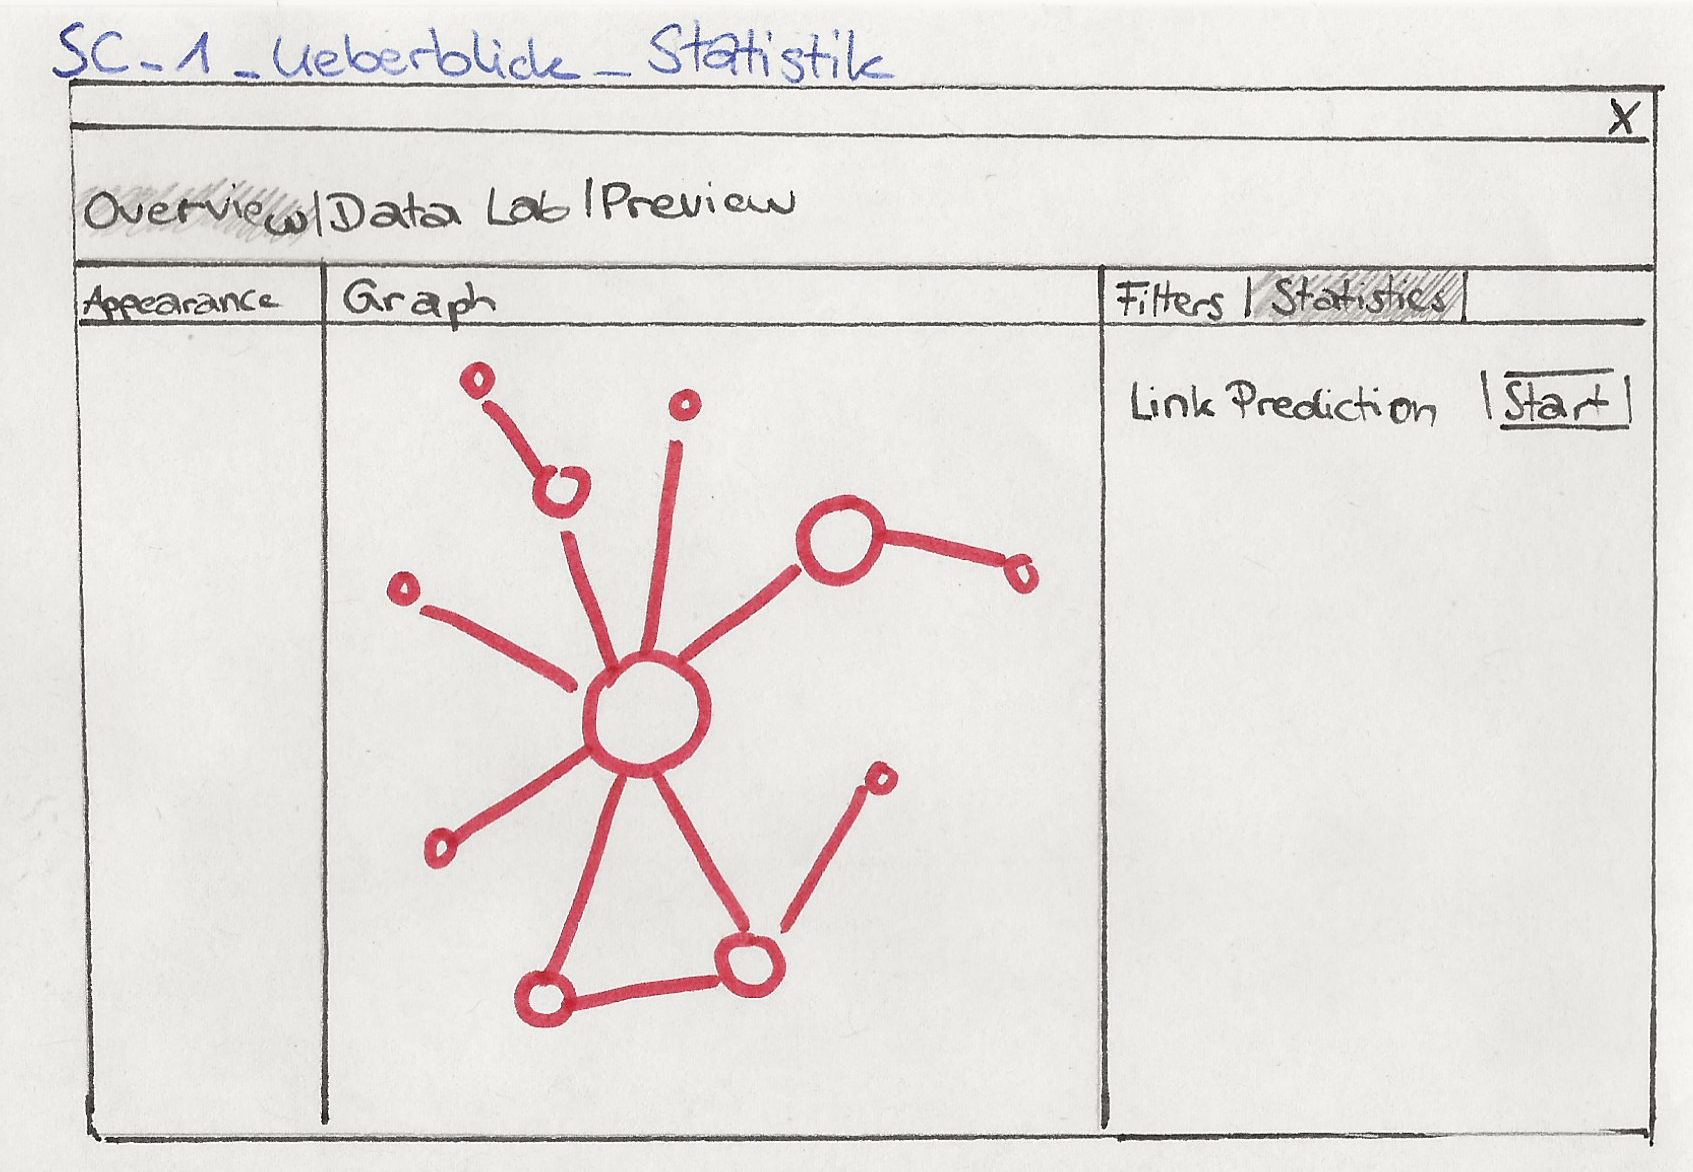
\includegraphics[width=\linewidth]{resources/SC-1.png}
    \caption{Überblick der Ansicht Statistik.}
    \label{fig:screen1}
\end{figure}

Im Bild kann man eine Skizze sehen, welche einen Überblick über den Aufbau von Gephi gibt. Grau hinterlegt sind die
angewählten Menü-Punkte. Unter dem Menü \textit{Statistics} wird hier nun ein Punkt "Link Prediction" mit einem
Start-Button eingefügt. In der Darstellung ausgelassen wurden die anderen Punkte, die bereits in diesem Menü existieren
wie beispielsweise "Average Degree".

\begin{figure}[htbp]
    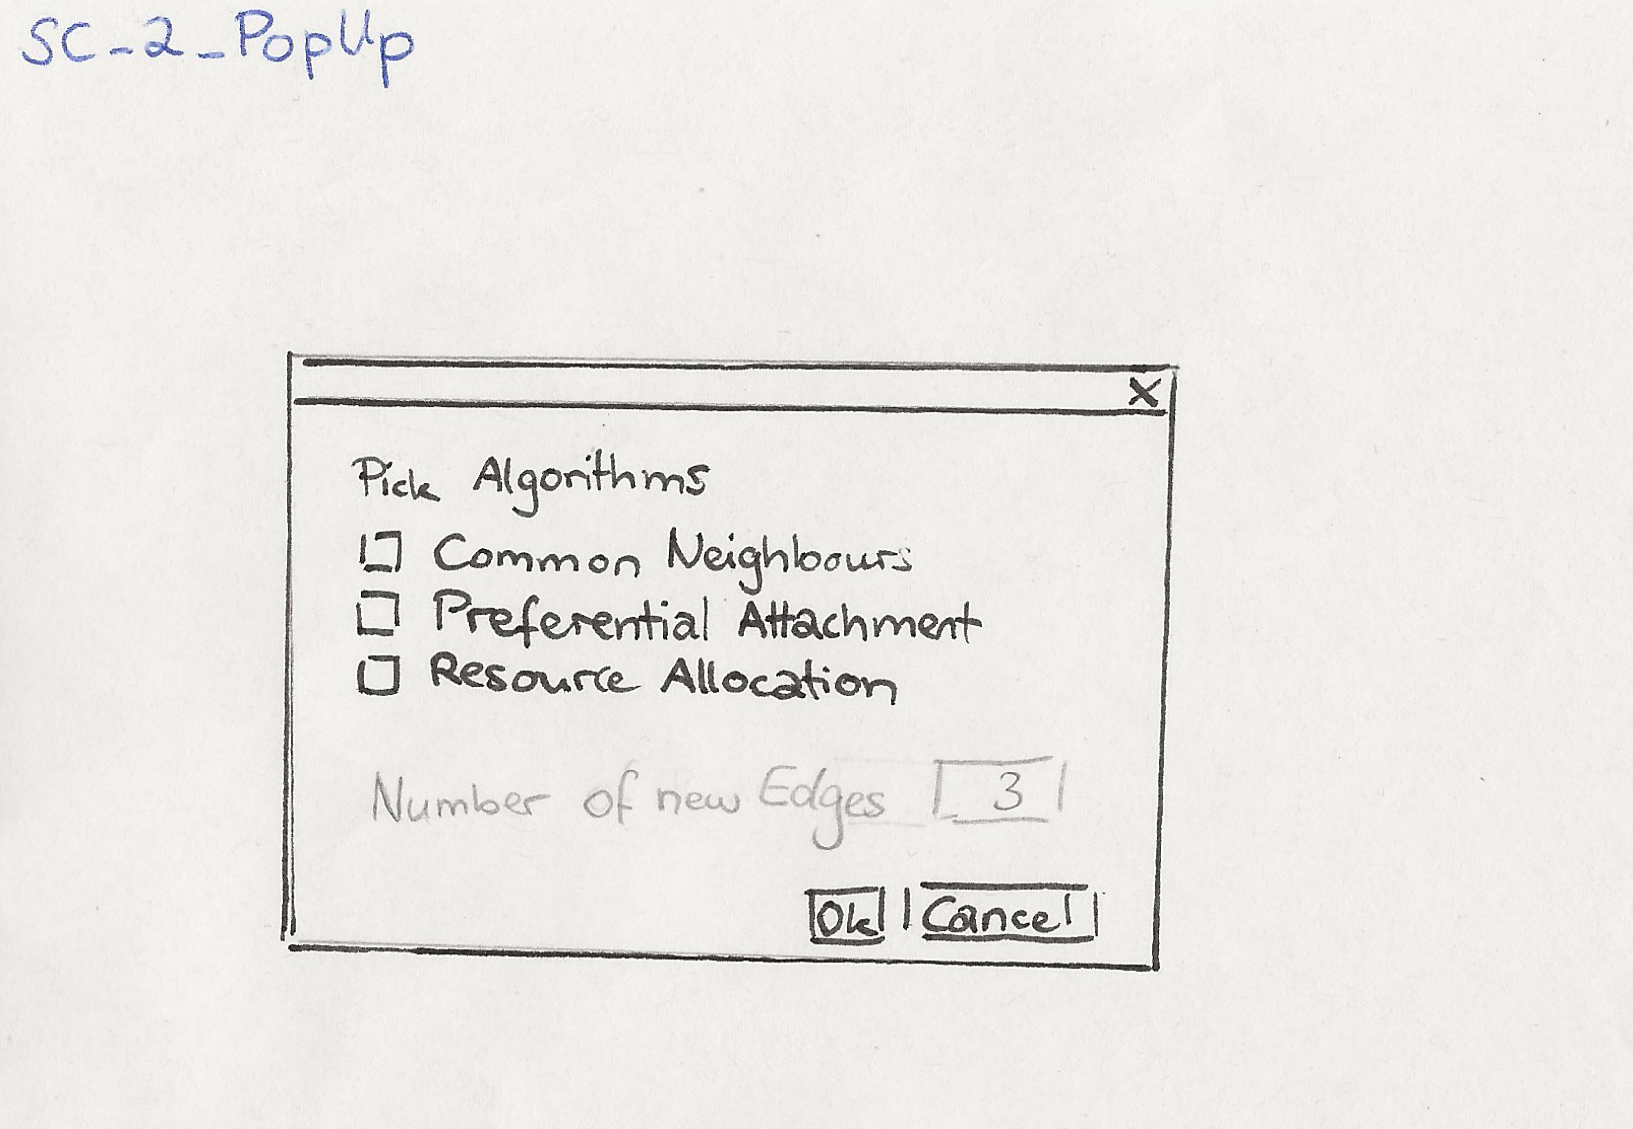
\includegraphics[width=\linewidth]{resources/SC-2.png}
    \caption{Pop-Up für die Auswahl der Berechnung.}
    \label{fig:screen2}
\end{figure}

Hier kann man sehen, dass beim Drücken auf "Start" ein Pop-Up geöffnet wird, in welchem man alle Algorithmen auswählen
kann, für welche die Link Prediction durchgeführt werden soll. In einem zusätzlichen Eingabefeld kann man einen Wert
von 1 bis x eingeben. Dieser besagt, wie viele Durchgänge bei der Link Prediction gemacht werden sollen - also wie viele
neue Kanten dem Graphen hinzugefügt werden.

Die Funktion der zusätzlichen Konfiguration eines Algorithmus ("advanced" Button) wird offen gehalten, wird aber für die
Implementierung des Common Neighbour und Preferential Attachment Algorithmus derzeit nicht benötigt.

Bei einer zu hohen Zahl oder der Auswahl bestimmter langwieriger Algorithmen soll eine Warnung an den User ausgegeben
werden. Wird diese bestätigt, so wird der Algorithmus trotzdem berechnet. Beim Abbruch kann der User seine gewünschten
Einstellungen verändern.

\begin{figure}[htbp]
    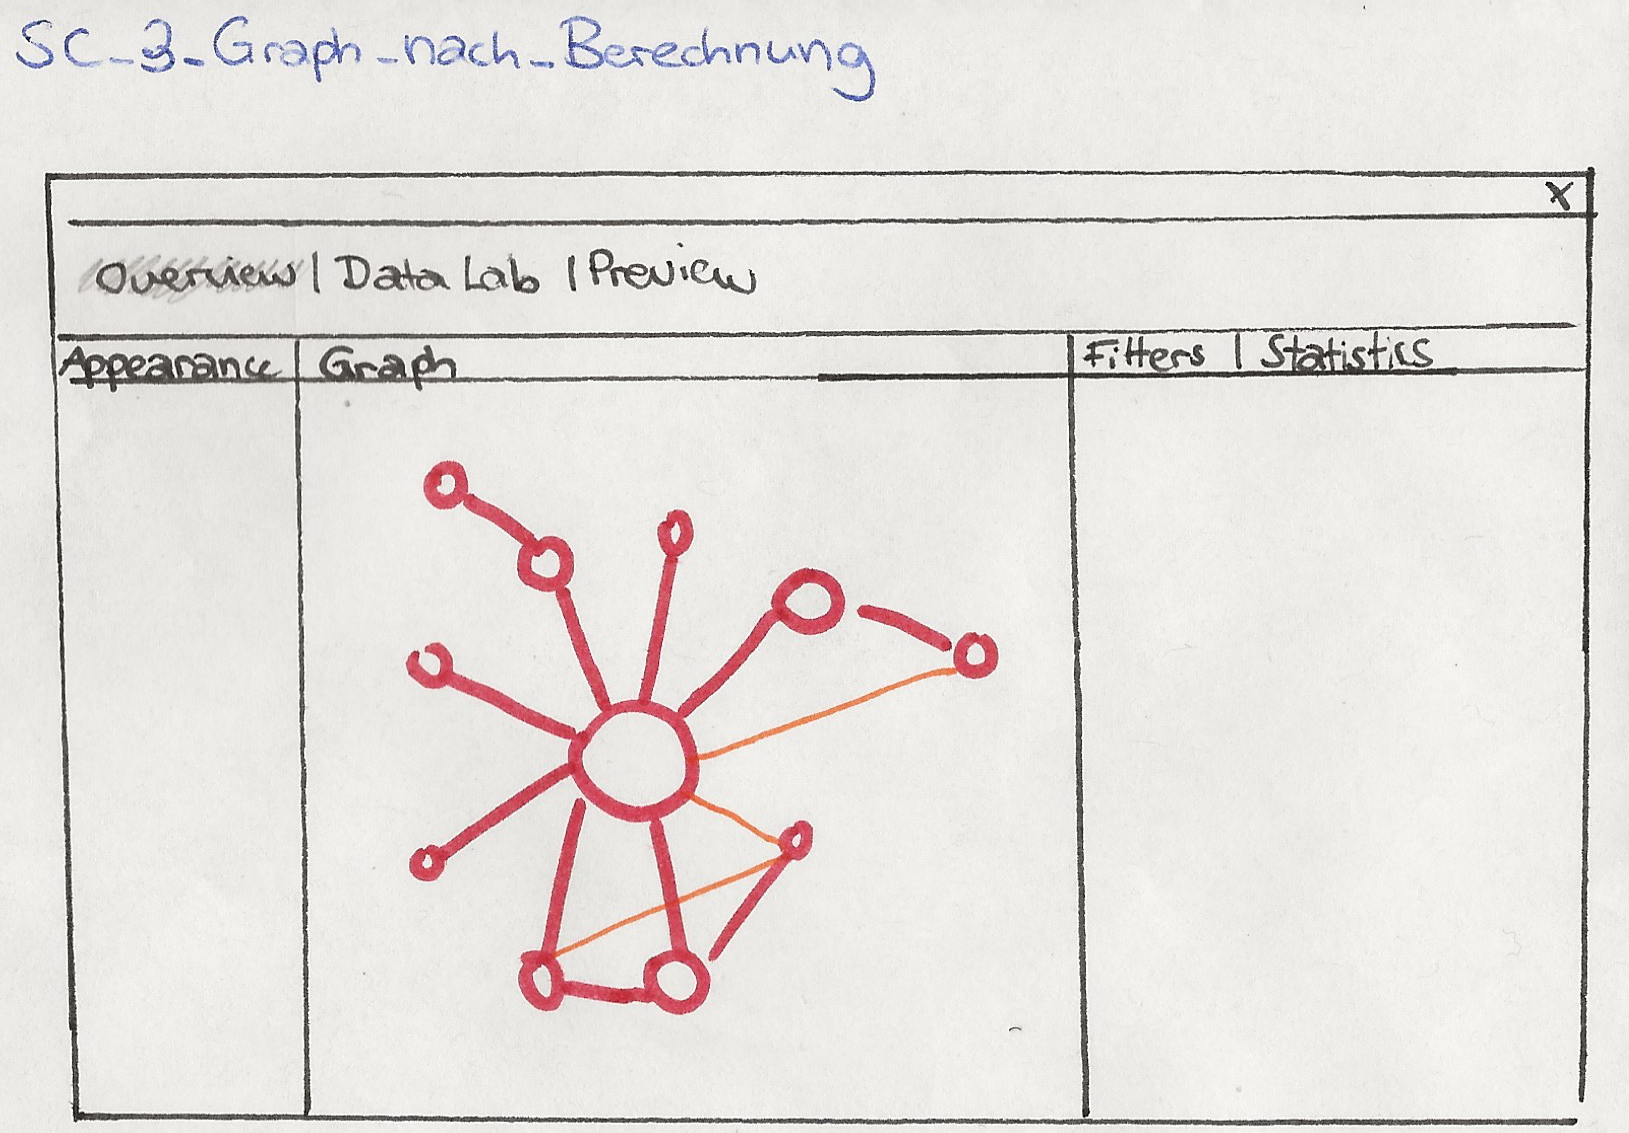
\includegraphics[width=\linewidth]{resources/SC-3.png}
    \caption{Modifizierter Graph mit vorhergesagtem Edge.}
    \label{fig:screen3}
\end{figure}

Im dritten Screen ist der Graph nach der Berechnung zu sehen. Es würden neue Kanten hinzugefügt. Diese können mit Hilfe
der Appearance Einstellungen eingefärbt werden, da im Data Laboratory Felder enthalten sind, die aussagen, ob eine
Kante mit einem Link Prediction Algorithmus hinzugefügt wurde oder ob sie bereits existiert hat.

\begin{figure}[htbp]
    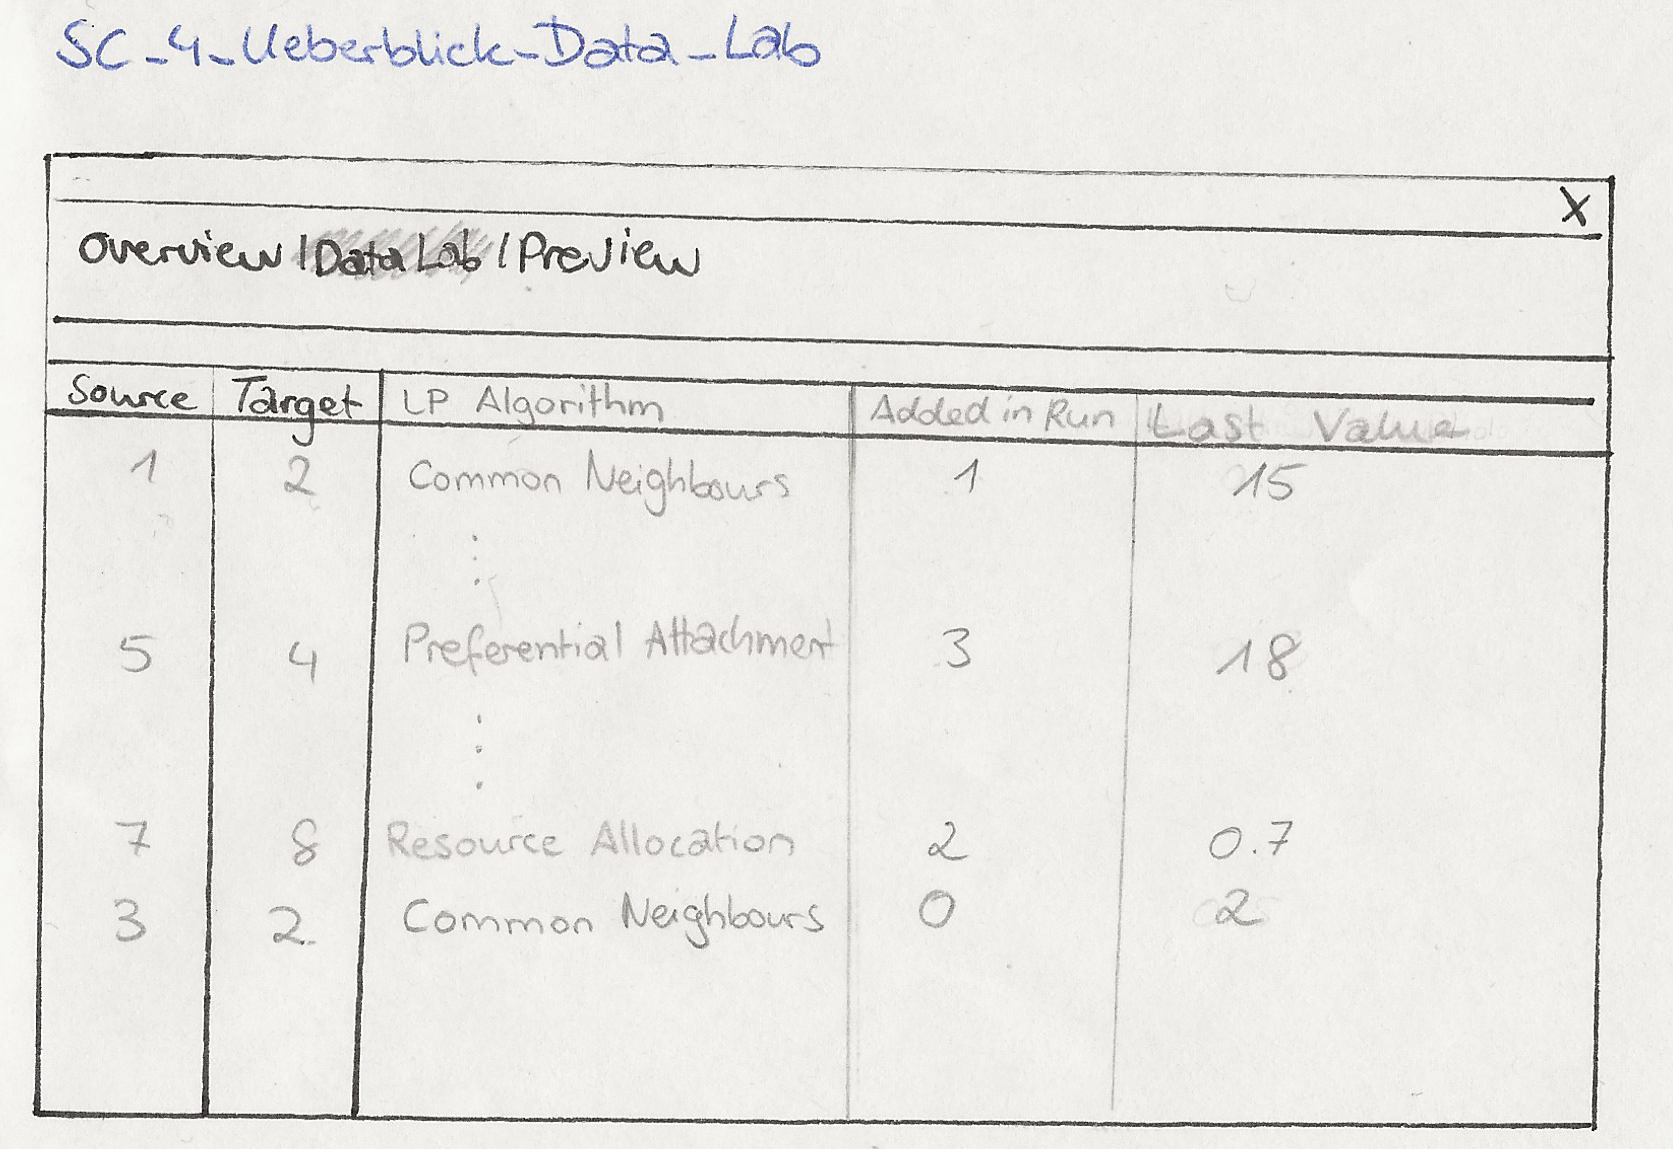
\includegraphics[width=\linewidth]{resources/SC-4.png}
    \caption{Data Laboratory mit neuen Edges.}
    \label{fig:screen4}
\end{figure}

In diesem Bild kann man die durch die Algorithmen neu hinzugefügten Attribute im Data Laboratory sehen. Diese sind auf
den Kanten des Graphen zu finden. Dort gibt es ein Feld "Link Prediction Algorithm", in welchem ein Wert enthalten ist,
um eindeutig zu zeigen, mit welchem Algorithmus diese Kante hinzugefügt wurde.

Eine weitere Spalte ist "Added in Run". Gibt der User bei der Berechnung den Wert 3 mit, so werden hier 3 Kanten pro
ausgewähltem Algorithmus durchnummeriert hinzugefügt. Damit der User einen Überblick hat, in welchem Durchlauf diese
Kante hinzugefügt wurde, haben wir dieses Attribut hinzugefügt. 1 würde dabei für die am wahrscheinlichsten hinzugefügte
Kante im ersten Durchlauf stehen, 3 für die wahrscheinlichste im dritten Durchlauf, usw.

Bei Kanten, die bereits vorhanden sind, werden Default Werte für die Spalten "Link Prediction Algorithmus" und "Added
in Run" eingefügt.

Die letzte Spalte "Last Threshold Link Prediction" ist eine optionale Spalte, bei der wir noch weitere Analysen
durchführen müssen, um zu evaluieren, ob diese einen tieferen Sinn hat. Hier würde zum Beispiel der letzte berechnete
Wert einer neu hinzugefügten Kante eingetragen werden. Dann wäre diese im Fall von keiner Berechnung, da die Kante
bereits existierte, ebenfalls mit einem Default-Wert befüllt.

\subsection{Filtern der neuen Link Prediction Kanten}

Die neu errechneten Link Prediction Werte sollen gefiltert werden können. Auch dazu wurden einige Skizzen erstellt.

\begin{figure}[htbp]
    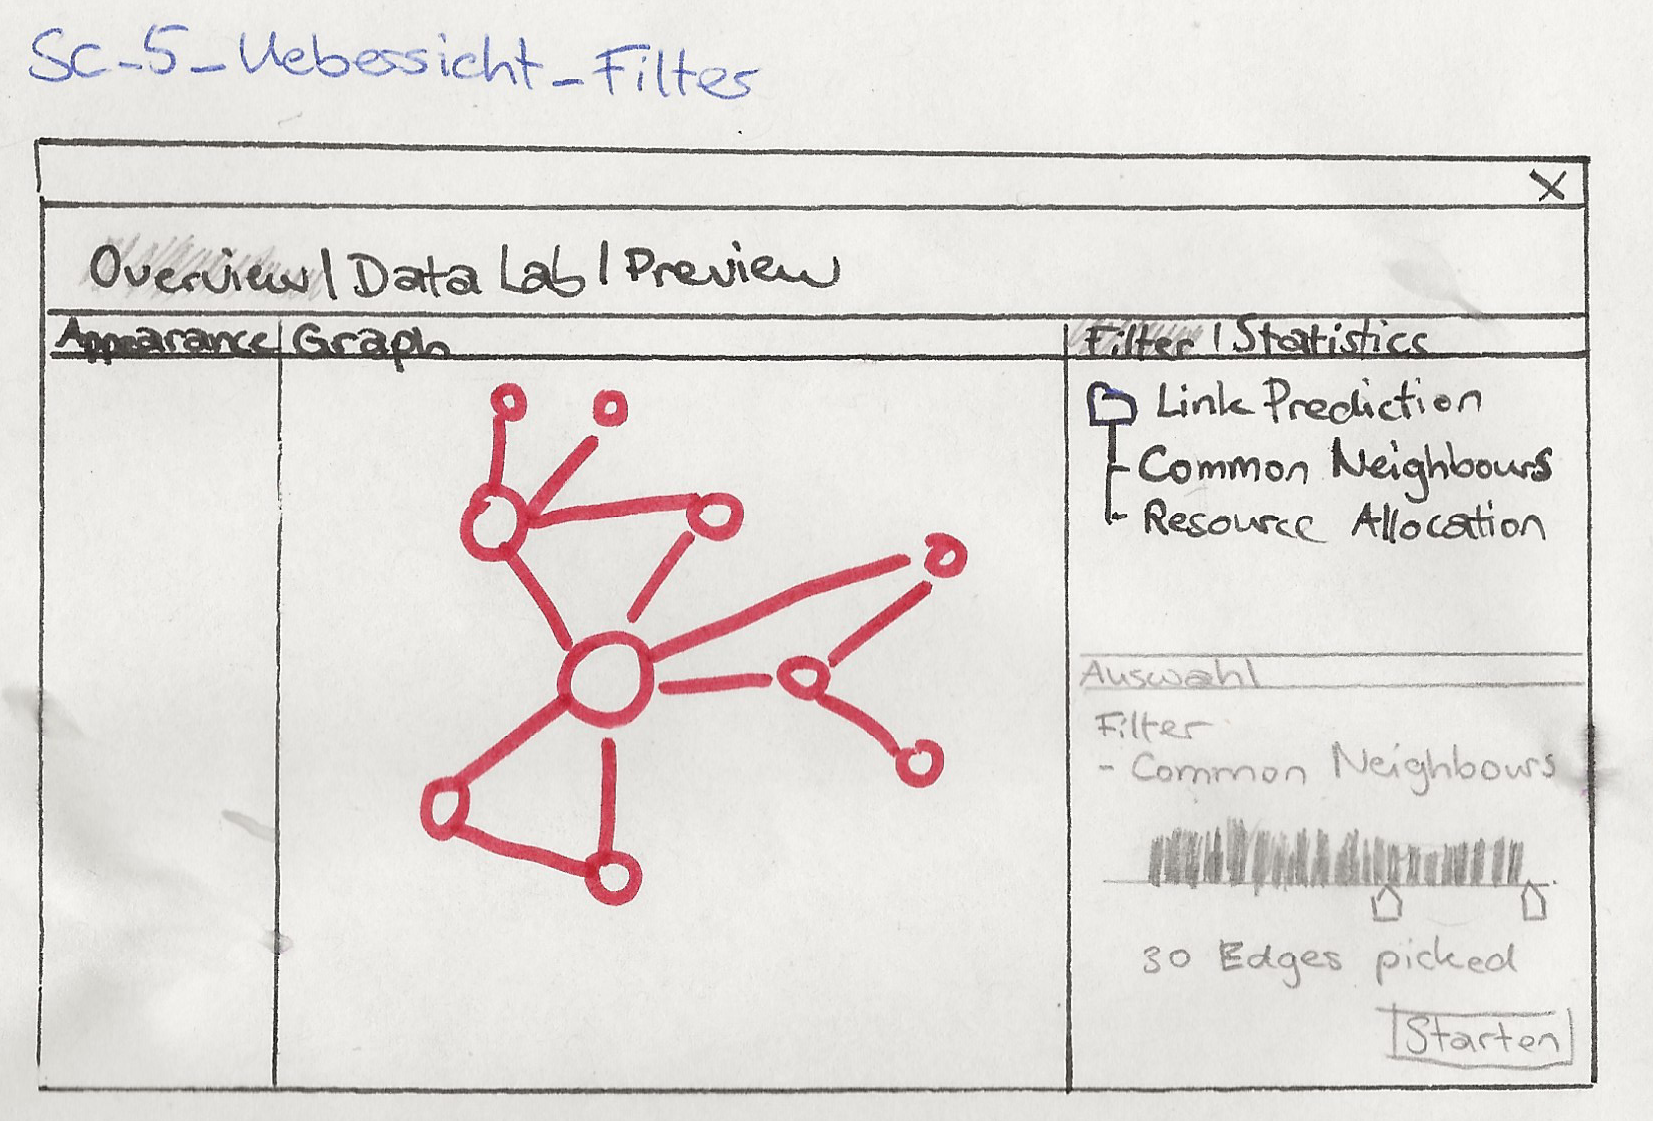
\includegraphics[width=\linewidth]{resources/SC-5.png}
    \caption{Überblick der Ansicht Filter.}
    \label{fig:screen5}
\end{figure}

Im Überblick ist zu sehen, wie der Link Prediction Filter in das bestehende GUI eingebunden wird. Dort wird es unter
\textit{Filter} einen neuen Ordner "Link Prediction" geben. Unter diesem können die Filter für einzelne Algorithmen
angewählt werden. Danach kann eingestellt werden, welche Links von welchen Durchläufen angezeigt werden sollen. Wird auf
"Start" geklickt, wird allenfalls das folgende Pop-Up angezeigt:

\begin{figure}[htbp]
    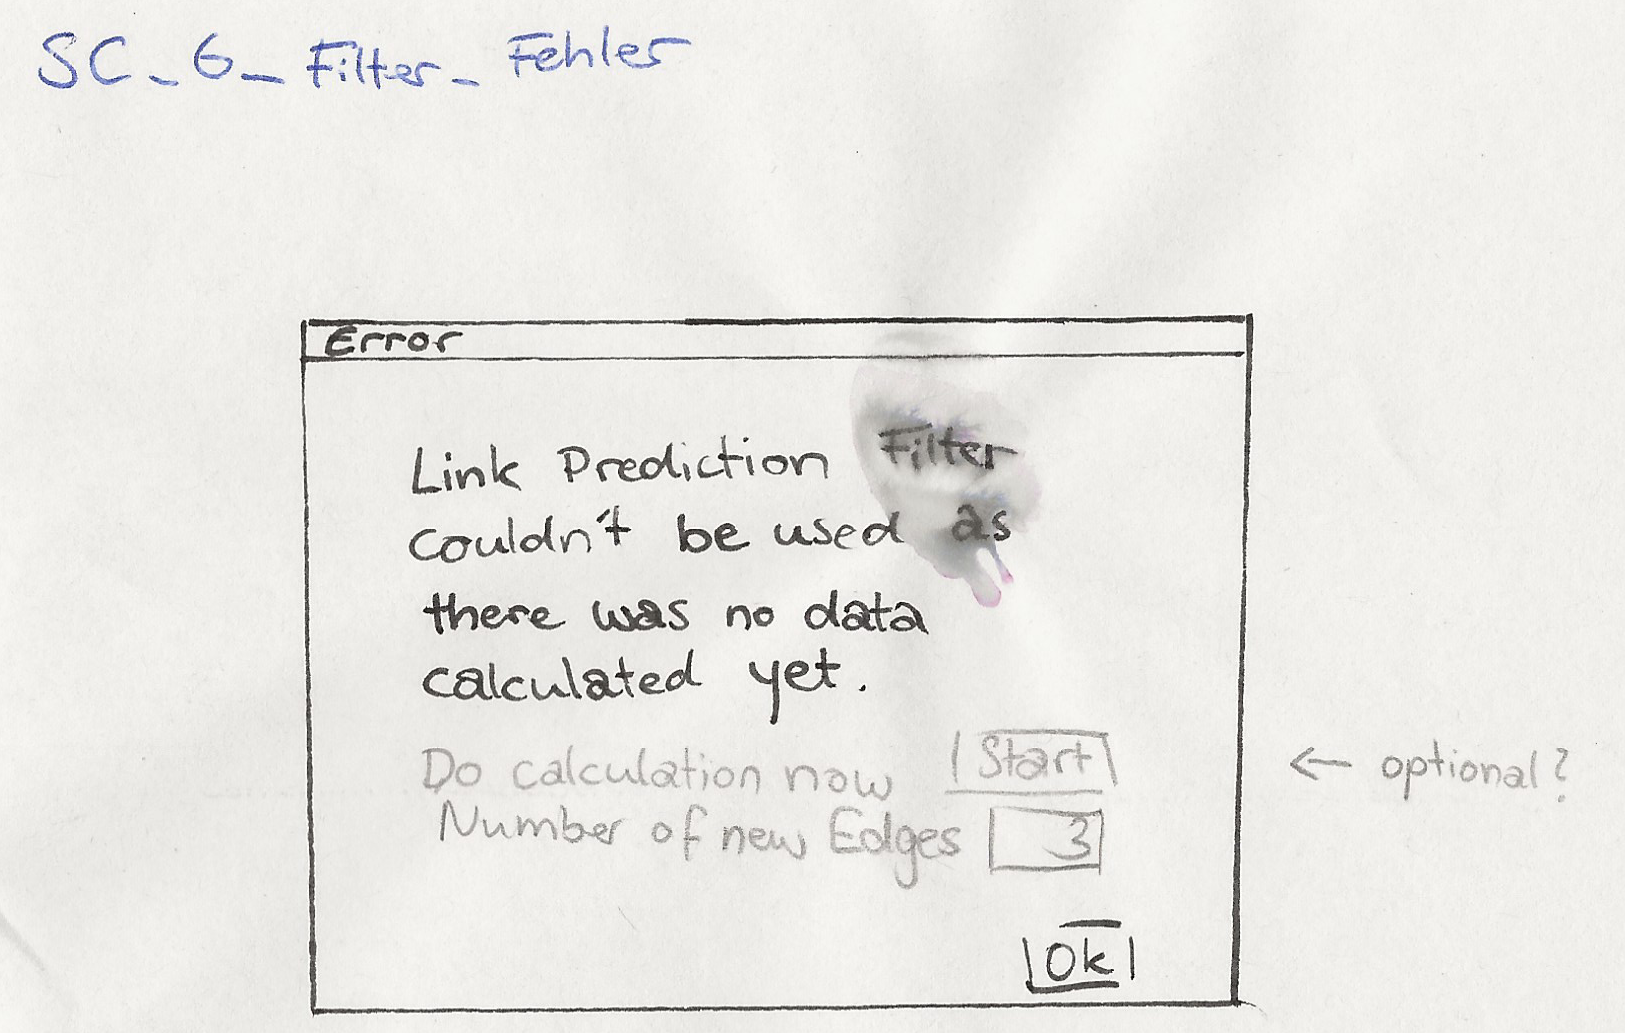
\includegraphics[width=\linewidth]{resources/SC-6.png}
    \caption{Fehlermeldung, wenn die Berechnung der Link Prediction noch nicht durchgeführt wurde.}
    \label{fig:screen6}
\end{figure}

Dieses Pop-Up stellt eine Fehlermeldung dar. Dort wird anstelle von "Link Prediction Filter" der ausgewählte Filter
stehen beispielsweise "Common Neighbour Filter" stehen. Diese Fehlermeldung erscheint, sofern die Berechnungen, um den
Filter anzuwenden, noch nicht ausgeführt wurden.

Optional behält sich das Projektteam vor, eine Option einzubauen, bei der direkt aus dem Fenster der Fehlermeldung die
Berechnung für diesen speziellen Algorithmus gestartet werden kann. Andernfalls kann die Fehlermeldung weggeklickt
werden und dann über die \textit{Statistics} die Berechnung vorgenommen werden.

\begin{figure}[htbp]
    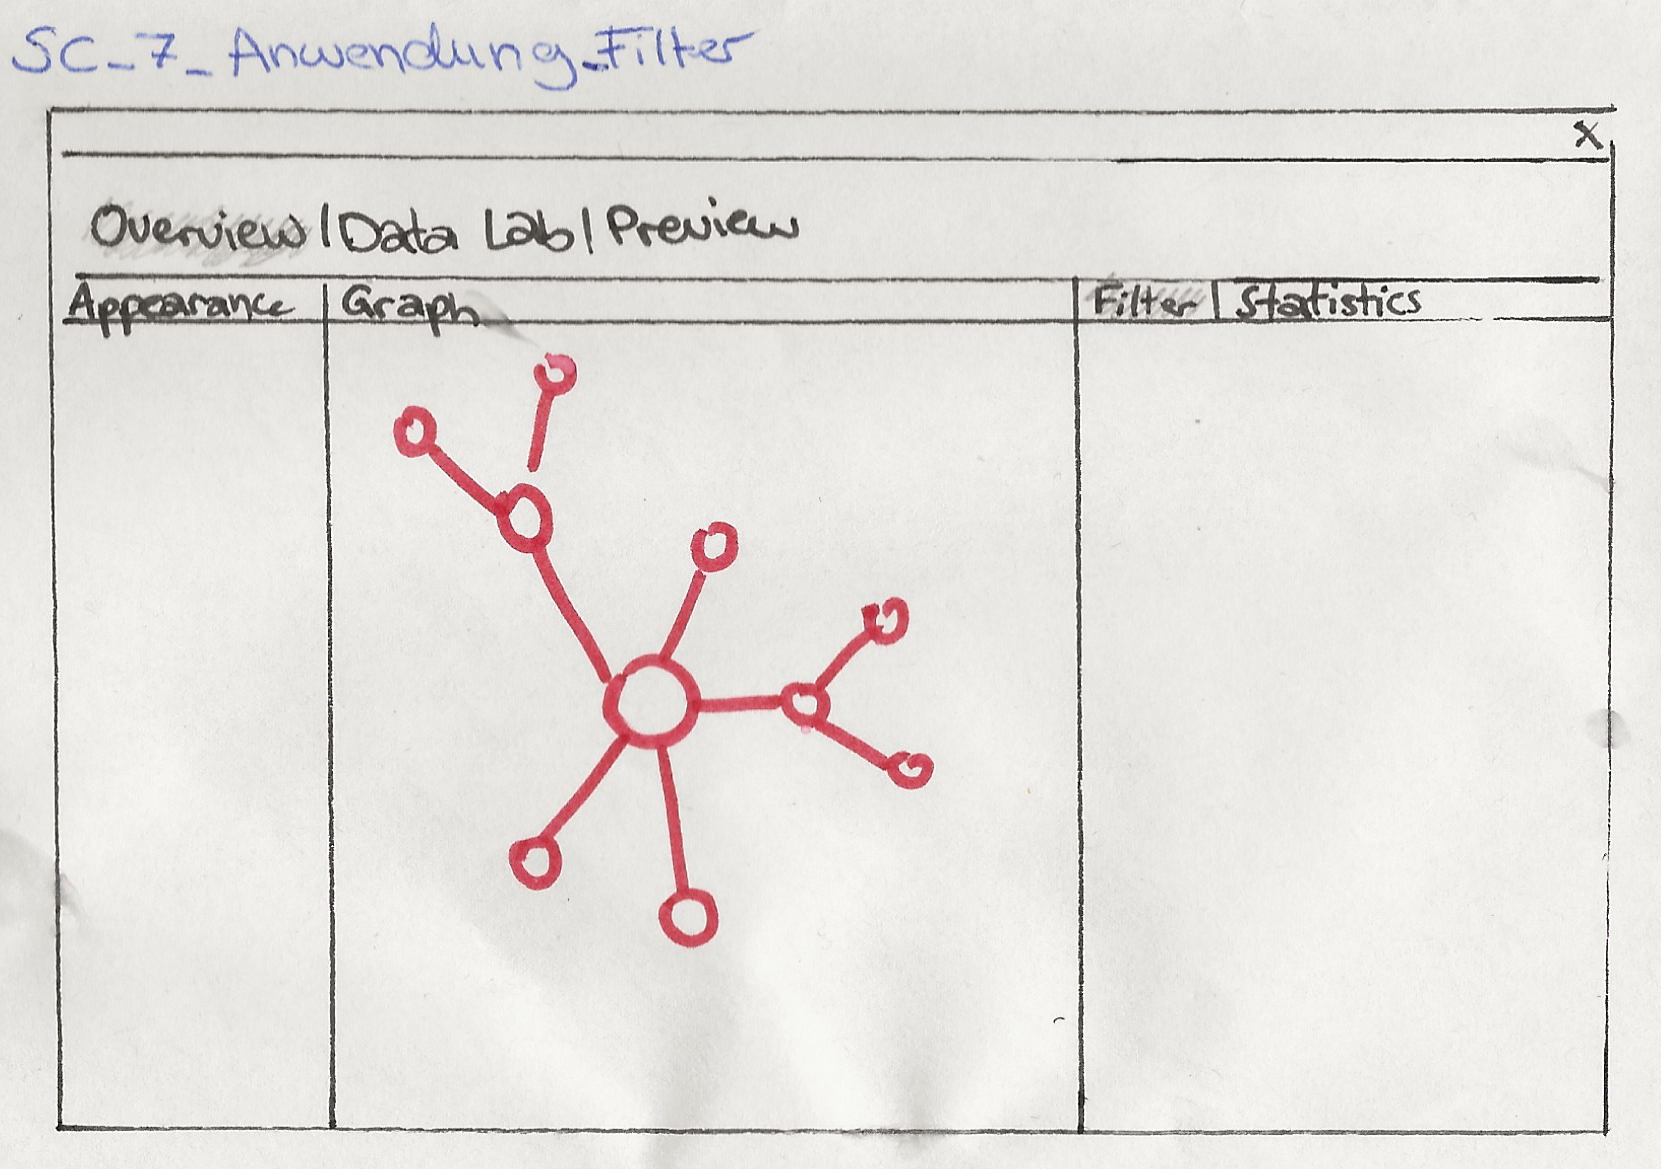
\includegraphics[width=\linewidth]{resources/SC-7.png}
    \caption{Gefilterter Graph.}
    \label{fig:screen7}
\end{figure}

Wurde der Filter angewendet, so wird der Graph dargestellt mit den neu ergänzten Kanten. Die bereits vor der Berechnung
eingefügten Kanten werden auch dann angezeigt, egal wie hier gefiltert wird.

\subsection{Vergleich der Link Prediction Algorithmen mit tatsächlichen neuen Links}

Dummy text.

\section{Link Prediction}

\subsection{Algorithmen (allgemein)}

Nach Recherche über die verschiedenen Algorithmen wurde entschieden, die Algorithmen "Common Neighbours" und
"Preferential Attachment" zu implementieren. Diese Entscheidung beruhte darauf, dass sich die beiden Algorithmen
insofern unterscheiden, dass beim Common-Neighbours-Algorithmus nur Knoten eine Rolle spielen, welche gemeinsame
Nachbarn aufweisen. Beim zweiten Algorithmus ist dies anders: Dort werden alle Knoten im Bezug aufeinander
berücksichtigt - hier ist also die Popularität eines einzelnen entscheidend, während beim ersteren Gemeinsamkeiten im
Vordergrund stehen.

Ausserdem wurde festgelegt, dass man sich in dieser Arbeit darauf beschränkt, die ungerichteten Graphen anzuschauen.
Die gewöhnlichen Algorithmen sind nicht spezifisch anwendbar auf gerichtete Graphen, so dass im Rahmen dieser Arbeit
auch diese als ungerichtet betrachtet werden. Eine Anmerkung diesbezüglich soll es bei der Link Prediction in Gephi
dementsprechend auch geben.

Die Begründung für diese Entscheidung beruht darauf, dass die Algorithmen, welche für gerichtete Graphen derzeit
entwickelt wurden, eine wesentlich höhere Komplexität aufweisen. Dies hätte dann einen Einfluss auf den vom Kunden
gewünschten Projektumfang - eventuell hätten dann Abstriche beim zweiten Teil des Projekts gemacht werden müssen.

\subsection{Algorithmus: Common Neighbours}

Der erste Algorithmus, welcher in diesem Projekt umgesetzt wurde, heisst Common Neighbours. Die Wahrscheinlichkeit
für das Entstehen eines neuen Edges wird bei diesem Algorithmus darüber berechnet, wie viele gemeinsame Nachbarn zwei
Knoten haben. Common Neighbours beruht daher auf dem Social Forces Prinzip der Homophilie, da die Wahrscheinlichkeit,
dass zwei Knoten sich verbinden, wenn sie Gemeinsamkeiten - also gemeinsame Freunde haben - grösser ist, als wenn nicht.

Die Formel für den Common Neighbours Algorithmus lautet, wie folgt:

common_neighbours(X,Y) = | N(X) \cap N(Y) |

Der Wert, der aus der Rechnung für diesen Algorithmus resultiert, ist also die Summe der Anzahl aller gemeinsamen
Nachbarn der beiden Nodes X und Y. Dieser Wert muss für alle Node-Kombinationen berechnet und anschliessend der höchste
Wert ausgewählt werden.

In Gephi ist die Berechnung dieses Werts bei den Statistiken unter Link Prediction zu finden. Die berechneten Werte
werden anschliessend im Data Laboratory gespeichert und können mit Hilfe von Filtern eingeschränkt werden.

\begin{figure}[htbp]
    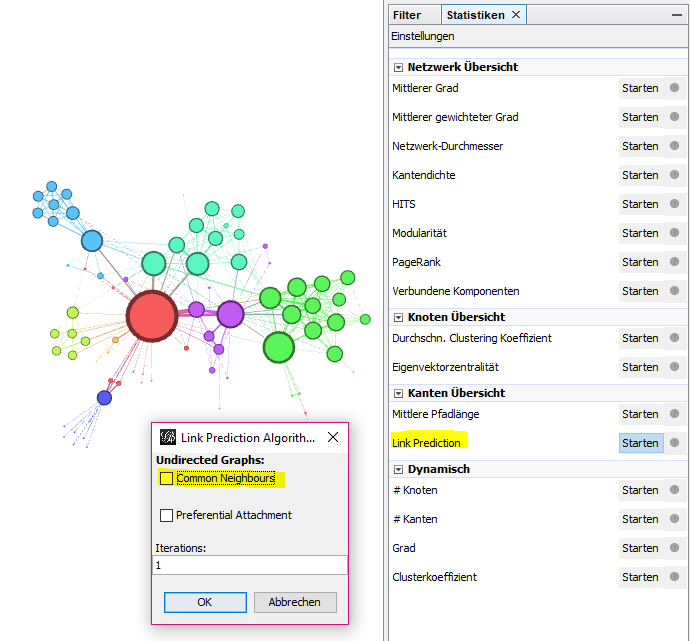
\includegraphics[width=\linewidth]{resources/gephi-CN.png}
    \caption{Gephi Common Neighbours Funktion.}
    \label{fig:screen8}
\end{figure}

\subsection{Algorithmus: Preferential Attachment}

Mit dem Preferential Attachment Algorithmus werden ebenfalls die Nachbarn berücksichtigt. Jedoch müssen diese nicht
mit den Nachbarn des anderen Knoten übereinstimmen - es geht lediglich um die Menge der eigenen Nachbarn. Die Entstehung
eines neuen Edges wird daher nicht über Homophilie bestimmt, sondern über Ansehen. Je mehr Nachbarn beide Knoten haben,
umso höher der resultierende Wert. Laut dieser Theorie ist die Wahrscheinlichkeit einen neuen Kontakt zu knüpfen
grösser, je grösser das eigene Netzwerk bereits ist.

Die Formel für den Preferential Attachment Algorithmus lautet, wie folgt:

preferential_attachment(X,Y) = | N(X) | \cdot | N(Y ) |

Der Wert, der aus der Rechnung für diesen Algorithmus resultiert, ist also das Produkt der Anzahl aller Nachbarn der
beiden Nodes X und Y. Dieser Wert muss für alle Node-Kombinationen berechnet und anschliessend der höchste Wert
ausgewählt werden.

In Gephi ist die Berechnung dieses Werts bei den Statistiken unter Link Prediction zu finden. Die berechneten Werte
werden anschliessend im Data Laboratory gespeichert und können mit Hilfe von Filtern eingeschränkt werden.

\begin{figure}[htbp]
    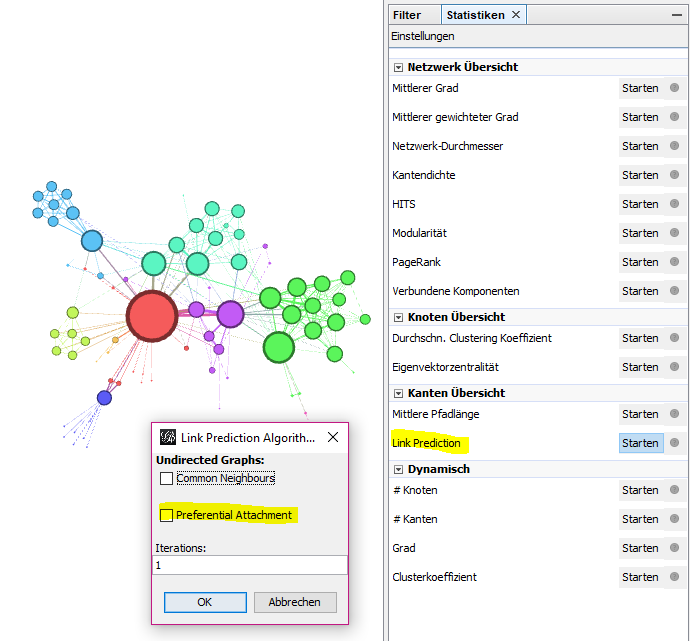
\includegraphics[width=\linewidth]{resources/gephi-PA.png}
    \caption{Gephi Preferential Attachment Funktion.}
    \label{fig:screen9}
\end{figure}

\section{Netzwerk- und Algorithmenvergleich}

Dummy text.